% Chapter 4

\chapter{Network Reconfiguration Software} % Write in your own chapter title
\label{Chapter 4}
\lhead{} % Write in your own chapter title to set the page header

% 4.1 Overview
% - Introduce the sections and the purpose/content of each section
\section{Overview}
This chapter discusses the software developed in this thesis. First, this chapter discusses the procedures involved in network reconfiguration and the features that this system needs to have to achieve that goal. Next, the features are discussed in terms of software functionality that needs to be implemented for those features to exist. Finally, the chapter discusses how the different functionality is grouped into software modules. The specifics of how each module works is described in Chapter 5.


% 4.2 Approach
% - Re-Summarize goal of the work (to design and implement a way to manage the re-configuration of WSNs)
% - State "thesis" -> that designed an approach that selects from the sensor network as if it were a database
% * you can represent the network as a database of abstract wisard deployments; describe what a wisard is
% * you can reconfigure the network by sending updates to sets of wisards

\section{Approach}
To achieve network reconfiguration functionality within WiSARDNet, a series of features need to be in place within the system. The features that are needed are as follows:

% a re-summarization o fthe goal of the thesis by describing the features it needs to have (the problem we are trying to solve)
\begin{itemize}
	\item A user needs to have an up to date understanding of a WSN's configuration.
	\item A user needs to have a way to specify the desired configurations or features they would like to make to a set or subset of WSN nodes.
	\item The user needs to be able to communicate their changes to the WSN. 
	\item The WSN needs to execute the new behaviors which the user has specified.
	\item The system needs to have built in protections which ensure continued WSN operation.
\end{itemize} 

As was shown in Chapter 2, there are a variety of ways that developers have used novel approaches to implement WSN reconfiguration functionality in their respective WSN platforms. For the work in this thesis, a database abstraction is used as the general approach to implementing WSN reconfiguration in WiSARDNet. The specific abstraction used, is the consideration that the WSNs in WiSARDNet can be viewed as a database of dynamic heterogeneous behaviors. By viewing the WSNs from a database perspective, queries and inserts become the language that users can use to interact with the WSN. The database paradigm is used to simplify the complexity of WiSARDNet and guide the design of WSN reconfiguration in WiSARDNet.\\

In addition to the database abstraction, another abstraction is used to approach WSN reconfiguration. In Chapter 3, all of the components that comprise a WiSARD are represented in the WiSARDNet PostgreSQL database as individual devices with deployments that describe their current state. Since a WiSARD is physically a collection of these devices, it is useful to represent the device deployments as WiSARD data objects. Figure \ref{fig:wisard_object} shows how the different components of a WSN node  can be described by a WiSARD data object. 

% wisard data objects
\begin{figure}[H]
	\centering
	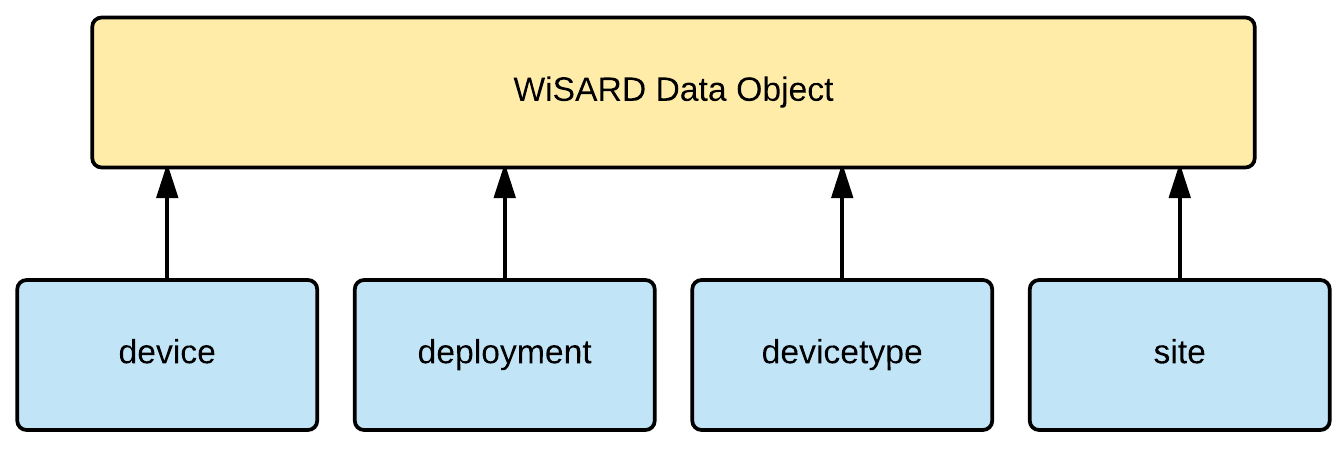
\includegraphics[width=\textwidth]{figures/wis_data_objects.png}
	\caption{A visual of the WiSARD abstraction which simplifies the view of a WSN node's many components}
	\label{fig:wisard_object}
\end{figure}

Using WiSARD data objects as an encapsulation of different device deployments means that a WSN can be reconfigured by updating sets of WiSARDs. The database abstraction of the WSNs and the WiSARD abstraction of the WSN node hardware components provide a conceptual foundation for the WSN reconfiguration features to be implemented in software.


% 4.3 Solution Design
% - Explain use cases for reconfiguration to illustrate what your solution will try to accomplish/will be used for
% - State explicit functionality that your thesis is adding: wisard selection, command validation, etc..
% - List the steps to select and reconfigure wisards end-to-end
% - Group functionality steps into modules/components
% - Show a "New" SEGA architecture diagram (add-on to figure 3.1) that highlights your additional modules/components
% - Explain Layer of objects and db code, specifically the Wisard class
\section{Solution Design}
Implementing WSN reconfiguration functionality in software into an existing software system requires that new code modules be developed whose features cover all of the desired use cases. A practical example might be the scenario where a researcher would like all soil moisture transducers attached to WSN nodes in a specific region to be sampled at twice their current sampling rate. Performing this procedure would involve the user specifying the region and sensor types needed to produce a matching set of WSN nodes and that they would like the sampling rate of those transducers to be changed. The software would need to validate that there are no conflicts between that user's requested changes and the existing operational configurations of other WSN nodes. Finally, the nodes would each be signaled in their respective WSNs via command packets and would then alert the user of the changes made.

\subsection{Implementing Functionality}
Each of the features described in the previous section needs to be specifically implemented as software functionality to be used in the WiSARDNet system. This section describes the software design for each feature. 

\subsubsection{Identification of WSN Nodes}
The first stage in reconfiguring a WSN is the specification of the node or nodes whose configurations will be modified. This operation can be completed by querying the network state information stored in PostgreSQL database tables. Transducer samples, sensor operational data, software profile information, and hardware meta-data are all stored within the database and are necessary to determine which nodes will need to be reconfigured. 

\subsubsection{Describing the New Configuration}
A WiSARD's task execution is governed by a set of configuration parameters stored within the device's non-volatile memory; this area of memory is called the task control block. Changing a device's behavior is achieved by overwriting specific values within the task control block, with values that represent different behaviors. The user must describe the changes to the system so that the correct fields in the task control block can be overwritten with appropriate values corresponding to the new behaviors. This is achieved by encoding different behavior or behavior profiles into control sequences which the WiSARDs are able to decipher. 

\subsubsection{Validating the New Configuration}
As the number of configuration changes and the number of affected WSN nodes increases, the opportunity for error or conflicts of interest between researchers and their assets also increases. To prevent conflicts, there is a need to validate that the intended changes will not interfere with the execution of other nodes in the network. This is achieved with user access control and command validation. User access control is the process of restricting the access of users to specific pieces of hardware or software based on a set of rules and permissions that govern the extent to which they can interact with the WSN. For example, a researcher should not be allowed to reconfigure another researcher's hardware or reconfigure the WSN in a way that will adversely affect other experiments. Command validation is the process of analyzing the intended changes and the state of the network, determining whether or not the the command is feasible as well as making sure the user  or process issuing the command has the appropriate permissions or membership access to the affected hardware.

\subsubsection{Signaling the WSN}
Once the commands are created, the specified nodes within the WSN need to be made aware of the desired changes. The command packets are added to MQTT messages and flushed from the MQTT broker at the data center to the destination garden server or servers. Each garden server has a WiSARD client which will retrieve the command packet from the local MQTT instance and send it into the WSN via the hub node. 

\subsubsection{Executing the Reconfiguration}
When a WiSARD receives a command message from a parent node, the WiSARD parses the command message and schedules a task to execute the command. Each WiSARD schedules tasks and executes them at the appropriate time. When a WiSARD executes a command, a report message is created and sent back through the network to the RTDC. The report message will confirm that the task was successfully executed or report that it failed, if the task did not execute successfully.

\subsubsection{Verifying the New Configuration}
Report messages that arrive at the RTDC are treated as data streams, the same way sensor readings or diagnostic data are. Reports are archived and made accessible.

After a change has been made and the report message has been sent back to the RTDC, these reports can be pulled and checked to verify that the changes specified by the user have been applied. After making a change, a WiSARD will report its status which then be reflected in the user's view of the network within their session once the data arrives back at the data center.

% software modules - WiSARD Browser, Command Generator, Validation
\subsection{Software Modules}
The software implementation of the functionality described in the previous section is grouped into three distinct modules:

\begin{itemize}
	\item WiSARD browser module
	\item Command generator module
	\item Validator module
\end{itemize}

The WiSARD browser module contains the functionality that can identify sets and subsets of WiSARDs that match a user's search criteria. Additionally, this module is responsible for providing an up to date view of a WSN.  The functionality which allows a user to describe a new WSN configuration and signal those changes to the WSN are grouped into the command generator module. The functionality which validates the safety of a new configurations, checks for conflicts, and implements user access control into the system are grouped into the validation module. With the addition of these three software modules, all of the funcionality necessary for network reconfiguration is in place. Figure \ref{fig:wisardnet_ci_updated} illustrates where these modules will fit into the WiSARDNet CI.\\

% wisardnet ci with additions
\begin{figure}[H]
	\centering
	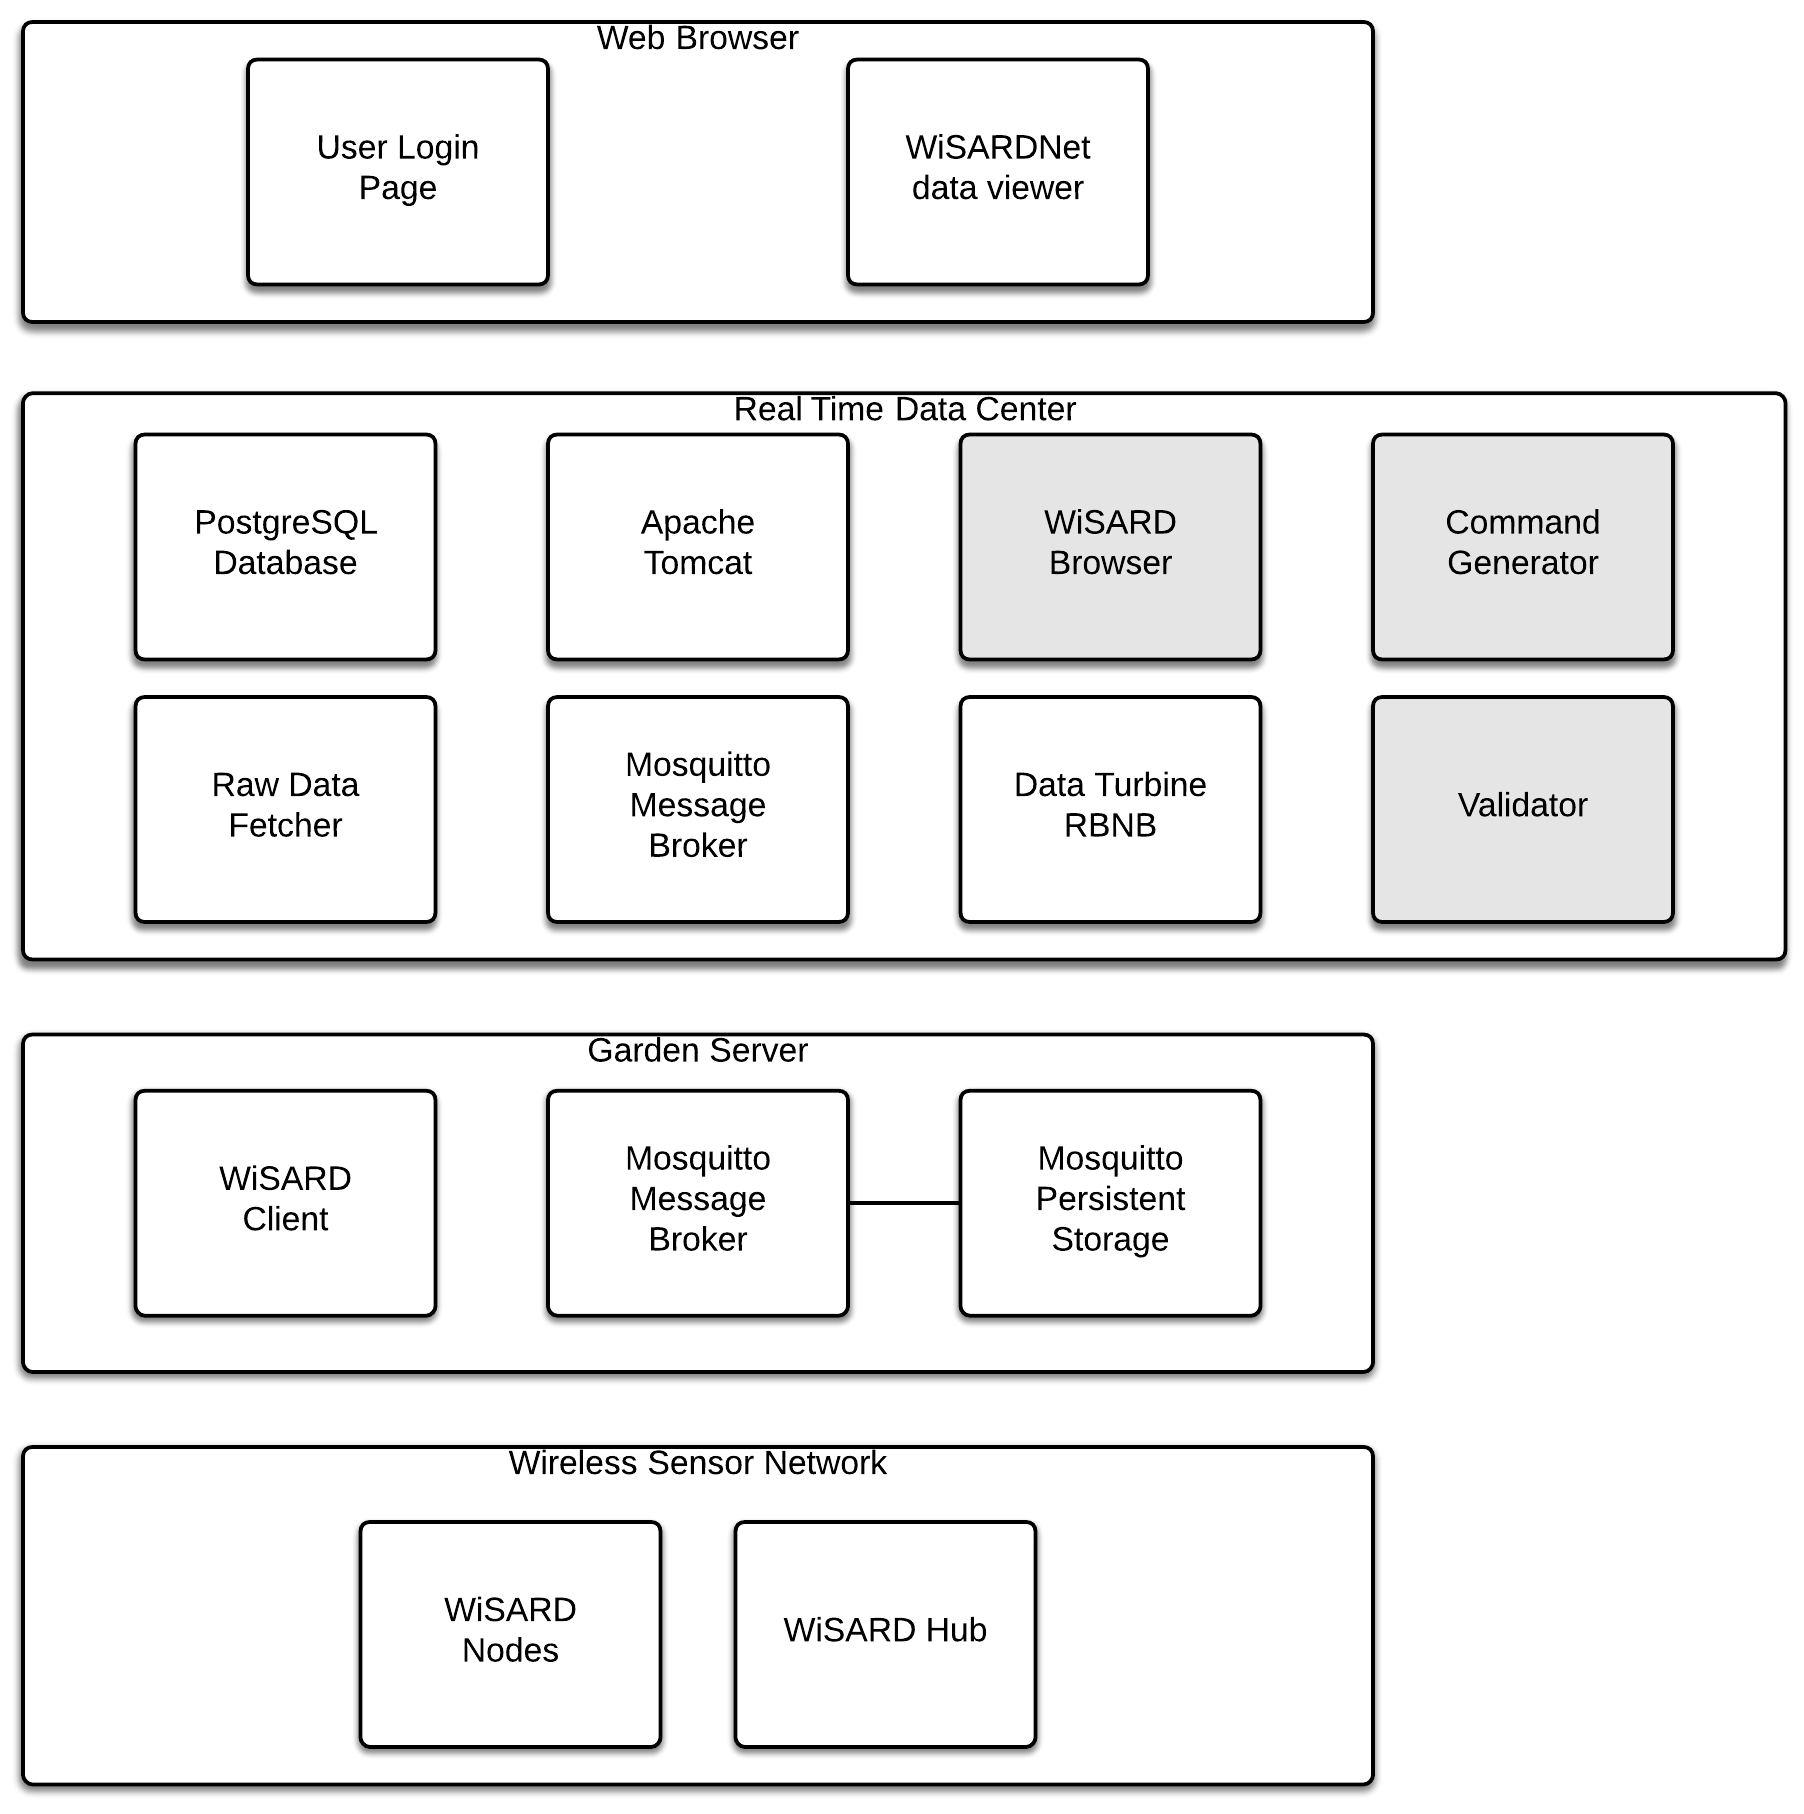
\includegraphics[width=\textwidth]{figures/wisardnet_ci_additions.png}
	\caption{A visual of where the new modules fit into the WiSARDNet CI}
	\label{fig:wisardnet_ci_updated}
\end{figure}

Each of these software modules contain separate functionality, but they all need to interact and share information with eachother as well as the other components of WiSARDNet. The WiSARD browser module needs to interact with the web portal user interface, it needs to gether information about the WSN nodes from the PostgreSQL database, and needs to be able to privide sets of WiSARDs to the other modules. The command generator module needs to be able to interact with the WiSARDNet web portal to generate commands based on a user's input. Additionally, it needs to access the list of WiSARDs that the WiSARD browser module produces. This module also needs to be able to access the PostgreSQL database to enable stored behaviors to be turned into commands. Lastly, this module needs to be able to provide information to the validator module so that the commands can be verified. The validator module needs to get session variables from the web portal to authenticate users. It also needs to be able to take in a set of commands from the command module, which is can validate and report its results.  To verify that users and commands are appropriate to execute on the network, they need to be analyzed against the user and access information stored in the PostgreSQL database.\\

In summary, all of the features necessary for WSN reconfiguration can be achieved by developing discrete pieces of functionality into the WiSARDNet CI. These pieces of functionality can be grouped into three distinct software modules: WiSARD browser, command generator, and validator. These modules need to be flexible and able to interact with the different components of the WiSARDNet CI as well as with eachother. The software implementation of each of the functional designs discussed in this chapter are discussed in Chapter 5.














%\section{Network Reconfiguration Stages}
%The reconfiguration of a WSN on this platform is accomplished through a sequence of operations:

%\begin{itemize}
%	\item Specify a set of WSN nodes to reconfigure
%	\item Specify the details of the desired changes to be made
%	\item Validate that the desired changes are allowed and do not create conflicts
%	\item Signal the network to perform the specified changes
%	\item Alert the user to the status of the changes
%\end{itemize}




%\section {Software System}
%	Devices, databases, systems (system architecture
%	- top-down architecture description
%	- section for each subsystem
%	- doesn't get super specific: subsystems: servlets, etc
%	- *show the layers or modules of the SYSTEM*

%This section gives a high-level systems-oriented overview of two subsystems that directly relate to network reconfiguration: user access control and the admin control subsystem.

%\subsection{User Access Control}
%The user access control subsystem is a software component which regulates the ability of different users to perform configuration changes on the WSNs within the WiSARDNet cyberinfrastructure. This subsystem acts a service which can provide validation of a specific user's requests, regulating their ability to proceed with actions they do not have permission to execute. It also interfaces with multiple other sybsystems. First, it needs to interface with the user interface subsystem; it filters a user's view of a WSN to only include nodes which a user has at least 'read' access for. Additionally, it needs to interface with the web portal admin control subsystem, which provides a suite of administrative tools that allow a user to view a WSN and its current configuration, signal changes to the WSN, and modify a WSN. By building this subsystem in such a way that it acts as a service to the other subsystems, it provides a generalized and scalable approach to controlling and regulating new subsystems and features which may be developed in the future. 

%\subsection{Admin Control}
%A core design philosophy of WiSARDNet is that it is a resource to enable researchers to effectively utilize and manage complex experimentation. The admin control subsystem describes the set of tools a user has to view and manipulate WSNs and experiments. This set of tools is governed by the user access control subsystem and therefore can provide a different user experience depending on the individual logged into the system. Each tool presents the user a set of features that enable WSN reconfiguration.\\ 

%The first tool is the WiSARD browser. This allows a user to query the network information tables within the database and see the current configuration of every WiSARD that they have access to view. WiSARDs are identifiable based on many different search criteria such as hardware identification numbers, SP board types, or deployment locations. It is important for a user to be able to filter lists of WiSARDs according to these criteria because the scope of desired changes may depend entirely upon a network's state with respect to that variable. For example, if a researcher wants to modify nodes between multiple sites equipped with a specific type of sensor then they need to be able to identify the set of nodes which match that criteria quickly to make the desired change.\\ 

%The second tool provided within the admin control subsystem is the WSN reconfiguration tool. This tool integrates with the WiSARD browser by taking a set of WiSARDs which the user specified and taking action to reconfigure them. This tool integrates with the user access control subsystem as well, because the WSN needs to be protected from changes that could adversely affect nodes and experiments outside of a user's ownership. The user access control subsystem filters which actions that the user is allowed to take in reconfiguring the sets of WiSARDs they retrieved from the WiSARD browser. Once a user signals an authorized action to be taken towards reconfiguring a WSN, this tool will build the messages that need to be sent to the affected WSNs where the commands can be scheduled and executed. At a high level, this process seems fairly straight forward, but actually accomplishing this within WiSARDNet requires a complicated set of interactions within the cyberinfrastructure. These interactions are described in detail in the following section.


%\section{Software Modules}
%The user access control and admin control subsystems provide users with the ability to observe and reconfigure WSNs but the software which implements these features relies heavily on a set of other software modules and services. This section discusses each software module in the system and how the features described in the previous section operate in practice. Figure \ref{fig:software_architecture} shows the software architecture of WiSARDNet that represents the work of this thesis.

% software architecture
%\begin{figure}[H]
%	\centering
%	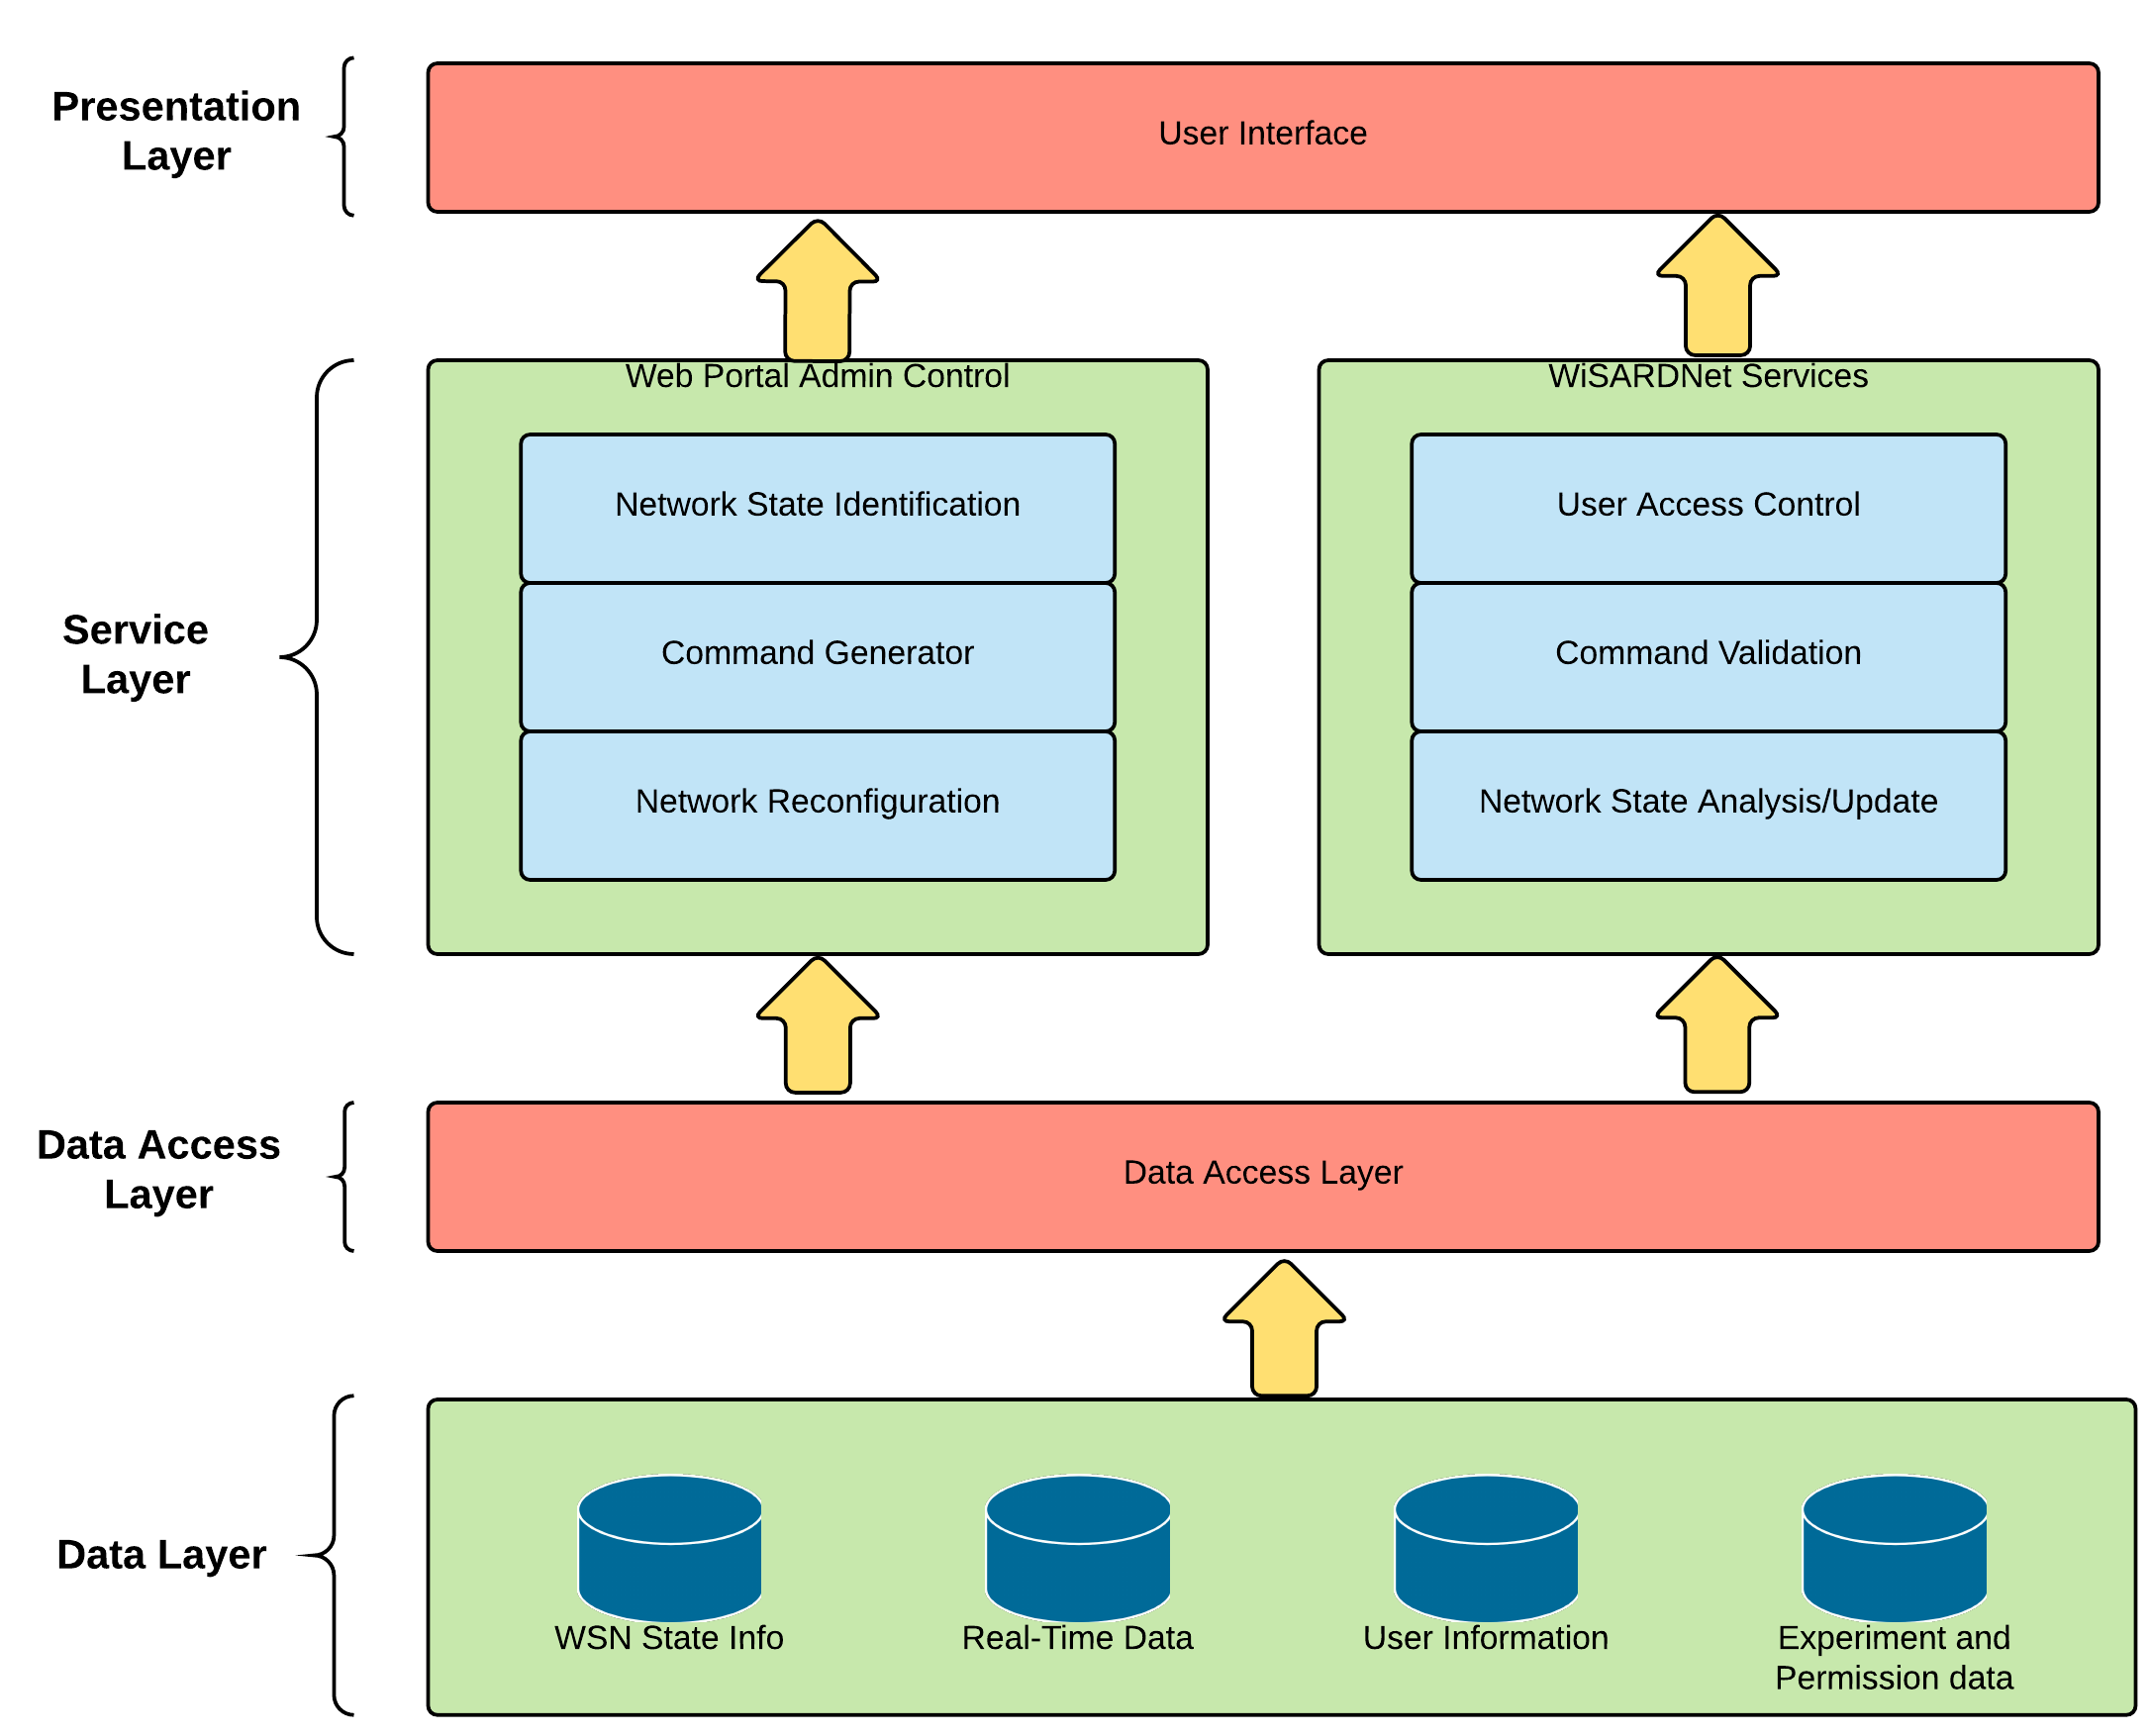
\includegraphics[width=\textwidth]{figures/software_architecture_diagram.png}
%	\caption{A visual representation of the software architecture that organizes the different software modules}
%	\label{fig:software_architecture}
%\end{figure}

% Servlet/JSP Interaction (software architecture)
%	- top - down architecture description
%	- section for each subsystem 
%	- describe the software layers/classes/modules
%	- look up typical jsp architecture descriptions
%	- show the code groupings (components) and their relationships (connectors)

%\subsection{User Interface}
%A user interface for the WiSARD browser and the configuration tool exists on a dynamic web page within the WiSARDNet web portal. This user interface is built with JavaServer Pages (JSP) and Java servlet technology which Apache Tomcat facilitates. JSP was chosen as the development platform for these tools because a large portion of the back-end cyberinfrastructe code was written in Java. Integration of new modules and application features into the existing system is significantly less difficult in this instance if they are written in Java. A jsp page with some javascript defines a single user interface for the user to use the WiSARD browser and network configuration tool.  Though the graphical user interface (GUI) for these tools exists within a single JSP page which defines the HTML code displayed by the user's browser, it interfaces with several servlets which form the back-end modules.\\

%A user that uses the GUI will begin by entering values to populate a series of forms in a JSP page with the search criteria that will help filter a set of WiSARDs from all of the WSNs. The user then submits their form to a servlet which will return the list  of WiSARDs to the JSP page. The procedure for specifying commands to execute and performing the reconfiguration follow the same pattern; the user fills out a form, sends the form to the servlet, and the servlet responds with a set of results which update the JSP page. The servlet directly handles getting information to and from the user via the JSP page, as well as delegating all of the complex computation operations to other modules. Figure \ref{fig:servlet_architecture} demonstrates how Apache Tomcat facilitates the interaction between the JSP page and the different servlets.

% servlet architecture
%\begin{figure}[H]
%	\centering
%	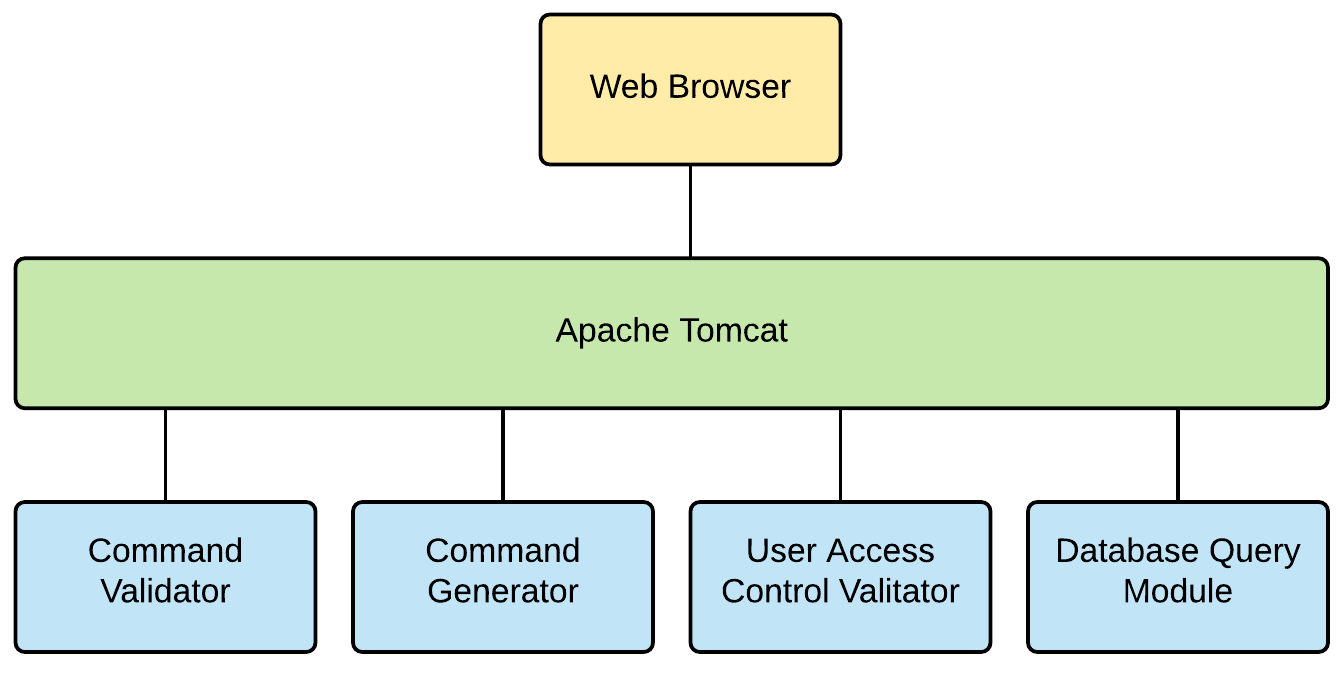
\includegraphics[width=\textwidth]{figures/servlet_architecture.png}
%	\caption{The organizational structure of the manner in which Apache Tomcat facilitates the interaction between the web browser and the servlet classes which provide critical application features}
%	\label{fig:servlet_architecture}
%\end{figure}


%\subsection{Database module}
%The database module is responsible for executing queries to the PSQL WiSARDNet database and returning data to the modules that use it. The database contains many different tables that each serve a vital purpose outside of simply storing transducer samples. All of the network state information that describes the network, user access and permission data, and CI networking information is stored in the database as well, making this a very robust and versatile module.\\

%\subsubsection{User Access Control}
%A large part of the user access control subsystem is managed by several tables in the PSQL database. The data schema for permissions was designed to be generic such that permissions can be applied to hardware, experiments, and software tools within the WiSARDNet web portal, as well as any future pieces of hardware and software that may be incorporated into WiSARDNet in the future. This was achieved by creating multiple abstractions that generalize users and WiSARDNet assets into two categories: permission entities and permission resources. A permission entity is a concept which describes any user, group, or organization that can be given permission to perform a task. A permission resource is a concept which describes any piece of hardware or software that an entity would need permission to use. With permission entities and permission resources clearly defined, a permission table with a single record maps an entity to a resource with a permission level. By implementing user access control in this manner, there is now a generalized way to grant permissions from a variety of entities to any kind of resource. Figure \ref{fig:user_access_control_tables} shows the references that connect each database table through foreign key constraints.

% user access control tables
%\begin{figure}[H]
%	\centering
%	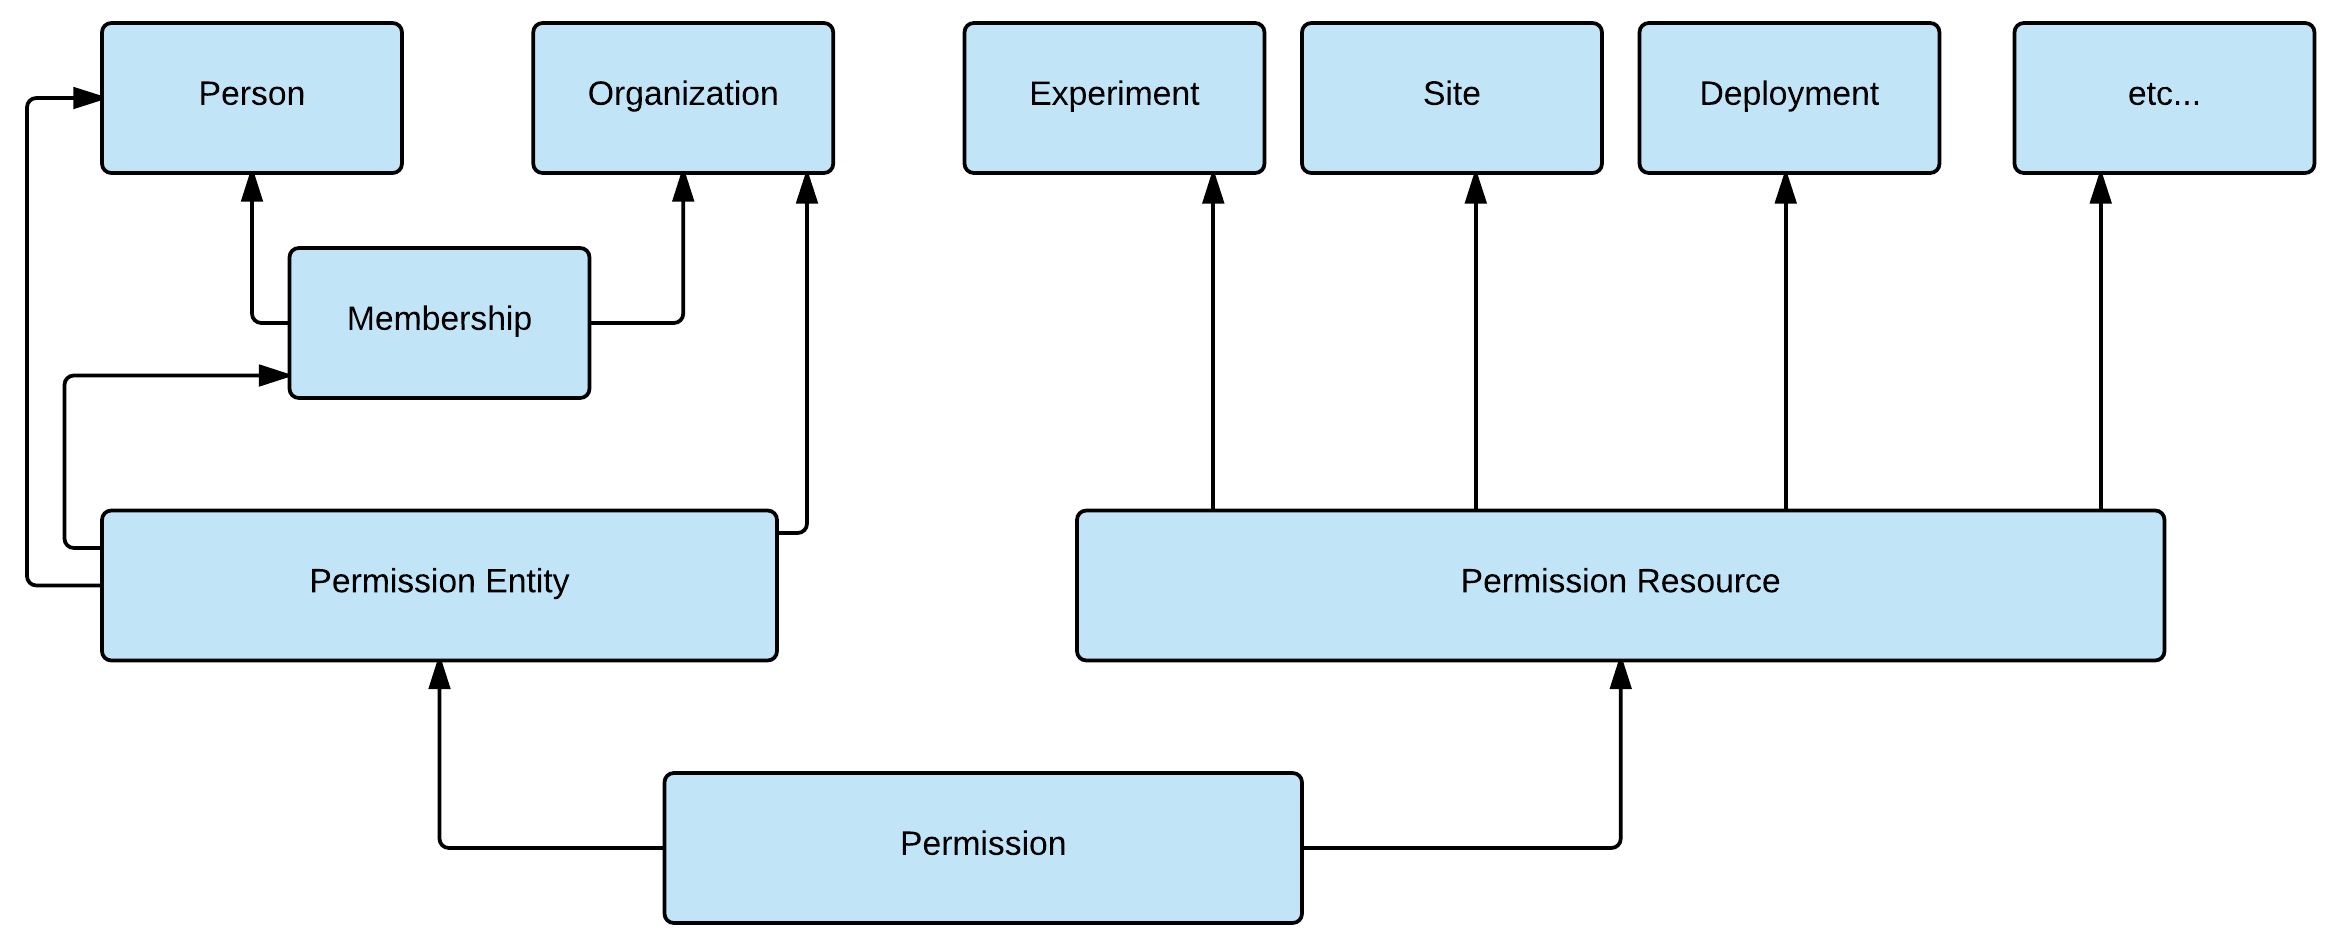
\includegraphics[width=\textwidth]{figures/user_access_control_schema.png}
%	\caption{A visual representation of the PSQL tables and their references which support the user access control paradigm}
%	\label{fig:user_access_control_tables}
%\end{figure}

%\subsubsection{WiSARD Data Objects}
%Chapter 3 discussed how device and deployment tables managed the specific implementation of a WSN node or a piece of hardware deployed into the field. A deployment record exists to record a specific instance of the device which it references. Data collected from one deployment of a device is a conceptually different piece of data than samples from another another deployment of that same device. WSN reconfiguration requires altering WiSARDs at the node level as individual transducers cannot be accessed directly. For this reason, the database module needs a way to select all of the relevant WSN node information as a WiSARD data object from the different PSQL tables. From the perspective of this data schema, a WiSARD can be thought of as a collection of active device deployments. Figure \ref{fig:wisard_object} shows how a WiSARD data object is created from the information stored in other tables. 

% wisard data objects
%\begin{figure}[H]
%	\centering
%	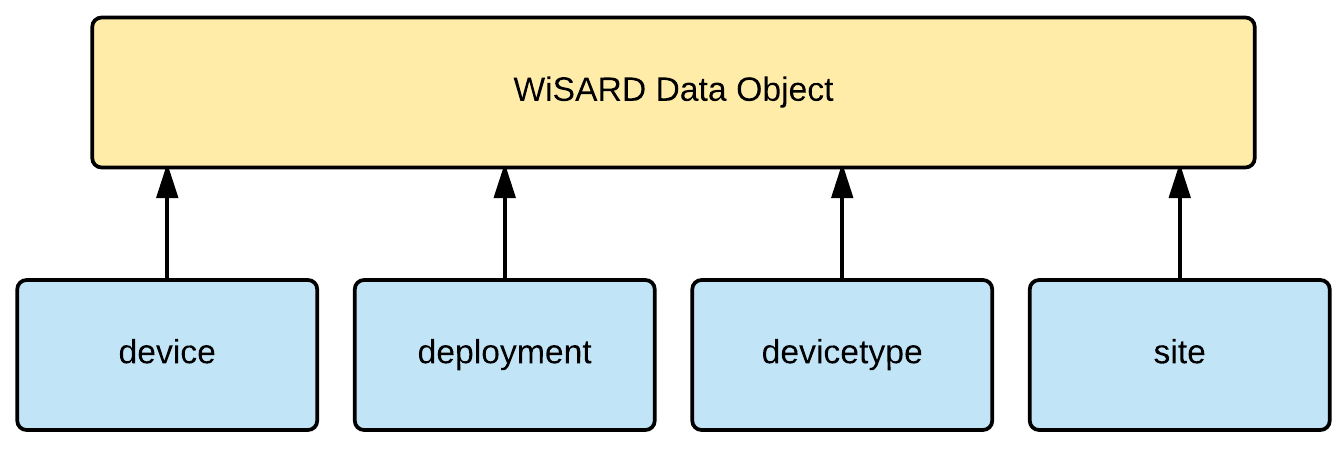
\includegraphics[width=\textwidth]{figures/wis_data_objects.png}
%	\caption{A visual of the database abstraction which simplifies the creation of WiSARD data objects}
%	\label{fig:wisard_object}
%\end{figure}

%\subsection{Command generation Module}
%Once a set of WiSARD data objects has been identified and the user has chosen which changes they would like to be made to the WSN, the command generation module needs to assemble command packets with information and task parameters that will allow WiSARDs to interpret. This is the software module which allows WSNs to be thought of as databases of heterogeneous behaviors. Different profile information describing new tasks can be queried from the database, updated with network state information, and then packetized.\\

%\subsection{Command generation Module}
%Once a set of WiSARD data objects has been identified and the user has chosen which changes they would like to be made to the WSN, the command generation module needs to assemble command packets with information and task parameters that will allow WiSARDs to interpret. This is the software module which allows WSNs to be thought of as databases of heterogeneous behaviors. Different profile information describing new tasks can be queried from the database, updated with network state information, and then packetized.\\

%\subsection{Validation Module}
%Following the creation of the commands but prior to sending them to the WSN, each command needs to be validated to ensure the user has adequate permissions to modify the affected nodes and that the commands are correct for the given set of WiSARDs. A user should not be able to send commands to modify nodes in ways they aren't capable of supporting or will negatively affect the WiSARDs without appropriate privileges. For example, a user should not be allowed to send a command that will change the WiSARD's software role to be a hub node, since hub nodes require special hardware connectivity and setup. Sending a command to perform that action would cause that node to stop sampling from its transducers and would orphan the node from the network such that no other commands can be sent to it. The validation module checks for potentially harmful commands such as this are filtered and prevented by the validation module before they are sent out to the WSN nodes.


%\subsection{Validation Module}
%Following the creation of the commands but prior to sending them to the WSN, each command needs to be validated to ensure the user has adequate permissions to modify the affected nodes and that the commands are correct for the given set of WiSARDs. A user should not be able to send commands to modify nodes in ways they aren't capable of supporting or will negatively affect the WiSARDs without appropriate privileges. For example, a user should not be allowed to send a command that will change the WiSARD's software role to be a hub node, since hub nodes require special hardware connectivity and setup. Sending a command to perform that action would cause that node to stop sampling from its transducers and would orphan the node from the network such that no other commands can be sent to it. The validation module checks for potentially harmful commands such as this are filtered and prevented by the validation module before they are sent out to the WSN nodes.


%\subsection{Network Configuration Module}
%The final module that completes the admin tool subsystem is the network configuration module. When a set of commands has been created by the command generation module and verified by the validation module, the network configuration model determines which garden servers commands need to be sent to and prepares them to be sent. Each garden server is accessible either via cellular or satellite modem, and therefore a separate TCP/IP connection must be made to each garden server separately. Getting the commands from the data center to the gardens servers relies heavily upon the Moquito MQTT broker. The software creates a new publisher client at the data center and encapsulates each command within an MQTT data message. The publisher client then publishes those messages to the MQTT broker of the garden server which the affected WSN resides. This process is then repeated for each garden server until all WiSARDs have been reconfigured.

%\section{Summary}
%Remote network reconfiguration is a complicated procedure and the WiSARDNet CI has many interacting software modules which make this possible. Efficient use of component abstractions, such as treating a WSN as a database of heterogeneous behaviors, helps to manage the complexity of complicated reconfiguration procedures.The different subsystems and software modules all interact to form a robust system that allows for a variety of control procedures which enable researchers to engage in complex remote experimentation.